% PCIM Europe 2027 -- synopsis
% Build (from this folder): latexmk -pdf PCIM_synopsis.tex
% Figures in figures/ are generated from the Python model in ../python:
%   python/venv/bin/python python/cycle_eval.py            (loss maps + cycle results)
%   python/venv/bin/python doc/figures/make_cycle_figures.py

\documentclass{PCIM-Abstract}

\usepackage{tikz}
\usetikzlibrary{positioning,calc,arrows.meta}
\usepackage{booktabs}
\DeclareSIUnit\rpm{rpm}
\DeclareSIUnit\pp{pp}
\DeclareSIUnit\ohm{\ensuremath{\Omega}}

\addbibresource{references.bib}

%mandatory fields
\title{AC Battery vs. Two-Level Inverter: Map and Drive-Cycle Efficiency from Passenger Cars to Trains}

\topicnumberandnames{H01 Power Electronics for E-Mobility}
\presentationform{Oral presentation}

\abstract{Battery-integrated modular multilevel converters (BI-MMCs), or AC batteries, replace the traction inverter with battery submodules switched by low-voltage Si MOSFETs. We present an open-source platform that compares the efficiency maps of a BI-MMC and a two-level SiC inverter, including MTPA operation and the battery, and evaluates their drive-cycle efficiency with SOC and temperature tracking. For six applications from cars to trains, the BI-MMC cuts semiconductor losses by \SIrange{26}{80}{\percent}, but its cells carry the phase current: it gains only about \SI{0.1}{\pp} where all energy is below base speed and loses up to \SI{1.7}{\pp} elsewhere.}

\begin{document}
\printtitle

\section{Synopsis}
In a conventional battery-electric drive, the pack is a single high-voltage string feeding a two-level (2L) SiC inverter that switches the full DC-link voltage at a fixed carrier frequency. The battery-integrated modular multilevel converter (BI-MMC), also known as an AC battery or modular multilevel battery \cite{lesnicar2003,helling2016,quraan2016}, instead distributes the cells over $N_\mathrm{sm}$ series-connected full-bridge submodules (SMs) per phase. Each SM inserts, bypasses or reverses its local cell string, so the phase voltage is synthesised directly from the batteries. This enables low-voltage Si MOSFETs with very low on-resistance, SM switching at a few times the fundamental frequency, and inherent cell balancing. The price is that the cells carry the switched phase current, including its reactive and field-weakening components, which raises the battery Joule losses \cite{kersten2019}.

Whether the BI-MMC is the more efficient drive therefore depends on where in the torque--speed plane a vehicle spends its energy. Published comparisons consider few operating points or one vehicle, or neglect the battery. This paper contributes:
(i)~an open-source evaluation platform that compares the efficiency maps of the two-level inverter and the AC battery over the full torque--speed plane, with identical machine, cells and installed energy, including the battery losses;
(ii)~a drive-cycle evaluation in the same platform, which steps through a duty cycle, tracks SOC and temperatures, and returns the cycle efficiency of both drives;
(iii)~a study of six applications, from passenger cars to off-road machines, ships and trains, which yields a simple rule for when an AC battery pays off.

\section{Evaluation Platform}
\Cref{fig:topologies} shows the two architectures. Each application in \cref{tab:apps} uses an interior PMSM ($p=4$) with the same per-unit parameters, the same \SI{24}{\ampere\hour} NMC cell, the Wolfspeed EDB005M12TM4 SiC module \cite{wolfspeed_edb005} with measured, current-dependent switching slopes and temperature-dependent $R_\mathrm{ds,on}$ for the 2L inverter, and \SI{0.3}{\milli\ohm} Si MOSFETs (four in parallel) switching at $f_\mathrm{c}=2f_\mathrm{e}$ in the BI-MMC. The cells per SM, $N_\mathrm{s,sm}$, are an input; $N_\mathrm{sm}=\lceil V_\mathrm{max}/(V_\mathrm{nom}N_\mathrm{s,sm})\rceil$ lets the BI-MMC reach the 2L phase voltage, with the same energy in both drives.

\begin{figure}[h]
\centering
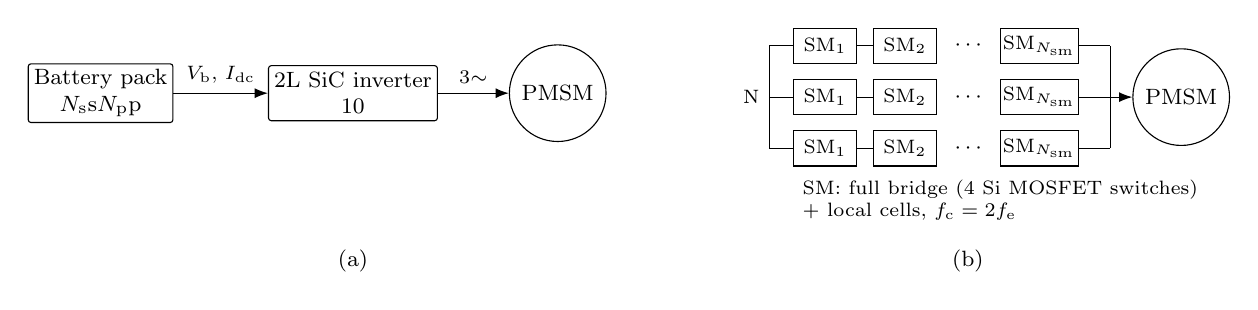
\begin{tikzpicture}[font=\footnotesize, >=Latex,
  blk/.style={draw, rounded corners=1pt, minimum height=7mm, align=center, inner sep=2pt},
  sm/.style={draw, minimum width=8mm, minimum height=4.5mm, inner sep=1pt, font=\scriptsize}]
  % (a) two-level
  \node[blk, minimum width=17mm] (pack) {Battery pack\\$N_\mathrm{s}$s$N_\mathrm{p}$p};
  \node[blk, right=12mm of pack, minimum width=17mm] (inv) {2L SiC inverter\\\SI{10}{\kilo\hertz}};
  \node[draw, circle, right=9mm of inv, minimum size=9mm] (m1) {PMSM};
  \draw[->] (pack) -- node[above, font=\scriptsize]{$V_\mathrm{b}$, $I_\mathrm{dc}$} (inv);
  \draw[->] (inv) -- node[above, font=\scriptsize]{3$\sim$} (m1);
  \node[font=\footnotesize] at ($(inv.south)+(0,-17.75mm)$) {(a)};
  % (b) BI-MMC
  \begin{scope}[xshift=92mm, yshift=6mm]
    \foreach \ph/\y in {a/0, b/-6.5mm, c/-13mm} {
      \node[sm] (s1\ph) at (0,\y) {SM$_1$};
      \node[sm, right=2mm of s1\ph] (s2\ph) {SM$_2$};
      \node[right=1mm of s2\ph] (d\ph) {$\cdots$};
      \node[sm, right=1mm of d\ph] (sn\ph) {SM$_{N_\mathrm{sm}}$};
      \draw (s1\ph) -- (s2\ph);
      \draw (sn\ph.east) -- ++(4mm,0) coordinate (o\ph);
      \draw (s1\ph.west) -- ++(-3mm,0) coordinate (n\ph);
    }
    \draw (na) -- (nc);
    \node[left=0mm of nb, font=\scriptsize] {N};
    \node[draw, circle, minimum size=9mm] (m2) at ($(ob)+(9mm,0)$) {PMSM};
    \draw (oa) -- (ob) -- (oc);
    \draw[->] (ob) -- (m2);
    \node[font=\scriptsize, align=left, anchor=north west] at ($(s1c.south west)+(0,-0.5mm)$)
      {SM: full bridge (4 Si MOSFET switches)\\+ local cells, $f_\mathrm{c}=2f_\mathrm{e}$};
    \node[font=\footnotesize] at ($(s2c.south)+(8mm,-12mm)$) {(b)};
  \end{scope}
\end{tikzpicture}
\caption{Compared architectures: (a) battery pack with a two-level SiC inverter; (b) BI-MMC with three star-connected strings of $N_\mathrm{sm}$ battery-integrated full-bridge submodules.}
\label{fig:topologies}
\end{figure}

\paragraph{Loss maps.} For every point of a $50\times100$ speed--torque grid covering motoring and regeneration, the stator currents follow from maximum-torque-per-ampere (MTPA) optimisation, solved with CasADi/IPOPT \cite{andersson2019} separately for each drive's voltage limit:
\begin{equation}
\min_{i_d,i_q}\; i_d^2+i_q^2 \quad \text{s.t.}\quad \tfrac{3}{2}p\big(\psi_\mathrm{f} i_q + (L_d-L_q) i_d i_q\big)=\tau_\mathrm{e}^*,\qquad v_d^2+v_q^2 \le \hat v_\mathrm{ph,max}^2(z),
\label{eq:mtpa}
\end{equation}
where $\hat v_\mathrm{ph,max}$ follows the cell open-circuit voltage at SOC $z$: $v_\mathrm{oc}N_\mathrm{s}/\sqrt3$ for the 2L inverter and $v_\mathrm{oc}N_\mathrm{s,sm}N_\mathrm{sm}$ for the BI-MMC. With peak current $\hat\imath$ and $N_\mathrm{p}$ parallel dies, the conduction losses are $\tfrac{3}{2}R_\mathrm{ds,on}(T_\mathrm{j})\hat\imath^2/N_\mathrm{p}$ (2L, iterated with the thermal network) and $3N_\mathrm{sm}R_\mathrm{ds,on}\hat\imath^2/N_\mathrm{p}$ (BI-MMC, two switches conduct per SM). Switching energies follow the slope-based method of \cite{graovac2006}, $E_\mathrm{sw}=\tfrac{1}{2}V\bar\imath\,(t_\mathrm{ri}+t_\mathrm{fv}+t_\mathrm{fi}+t_\mathrm{rv})$, with $V$ the DC-link or SM voltage. The cells are SOC-dependent first-order equivalent circuits. The 2L pack carries only the active-power current $I_\mathrm{dc}$; in the BI-MMC, the cell current is the phase current gated by the unipolar PWM state $s(t)\in\{-1,0,1\}$ and simulated in the time domain:
\begin{equation}
i_\mathrm{b}(t)=s(t)\,i_\mathrm{ph}(t),\qquad \frac{\mathrm{d}v_{C}}{\mathrm{d}t}=\frac{1}{C_1}\Big(i_\mathrm{b}-\frac{v_C}{R_1}\Big),\qquad P_\mathrm{b}=\big\langle R_0 i_\mathrm{b}^2+v_C^2/R_1\big\rangle_{T_\mathrm{e}} .
\label{eq:batt}
\end{equation}

\paragraph{Duty cycles.} Road and rail speed profiles are converted to machine speed and torque with a road-load model $F=k_\mathrm{m}m\dot v+\tfrac12\rho c_\mathrm{d}Av^2+c_\mathrm{rr}mg$ (Davis resistance for the train), the wheel radius and a gear ratio. The truck (\SI{40}{\tonne}) drives the \SI{119}{\kilo\metre} Södertälje--Norrköping road with its measured slope profile, the off-road machine follows the NRTC, and the ship the four propeller-law modes of ISO 8178 E3. $P_\mathrm{b}$ and the gear ratio are sized so that each cycle stays within the torque and power limits. Instead of interpolating the maps, the evaluator steps through each cycle: at every sample it solves \cref{eq:mtpa} at the present SOC, evaluates the loss models of both drives, updates SOC from the charge drawn per cell and evaluates a steady-state thermal network for the junctions, cases and cells. Torque beyond the common envelope of both drives is assigned to the mechanical brake. The cycle efficiency is $\eta_\mathrm{cyc}=1-E_\mathrm{loss}/(E_\mathrm{mot}+E_\mathrm{reg})$.

\begin{table}[h]
\centering
\caption{Applications, duty cycles and cycle efficiency at \SI{50}{\percent} SOC (semiconductors and battery). $\Delta\eta=\eta_\mathrm{BI}-\eta_\mathrm{2L}$; the range in brackets covers \SIrange{20}{90}{\percent} SOC.}
\label{tab:apps}
\footnotesize
\setlength\tabcolsep{3pt}
\begin{tabular}{@{}lrrrrclrrr@{}}
\toprule
Application & $P_\mathrm{b}$ & $V_\mathrm{dc}$ & $E_\mathrm{b}$ & $n_\mathrm{b}$ & $N_\mathrm{sm}\times N_\mathrm{s,sm}$ & Duty cycle & $\eta_\mathrm{2L}$ & $\eta_\mathrm{BI}$ & $\Delta\eta$ \\
 & [\si{\kilo\watt}] & [\si{\volt}] & [\si{\kilo\watt\hour}] & [\si{\rpm}] & & & [\si{\percent}] & [\si{\percent}] & [\si{\pp}] \\
\midrule
Passenger car & 150 & 400 & 75 & 5000 & $9\times7$ & WLTC Class 3b \cite{gtr15} & 98.87 & 98.38 & $-0.49$ \scriptsize{[$-0.77$, $-0.34$]} \\
City bus & 350 & 700 & 350 & 2500 & $11\times10$ & Braunschweig \cite{drivecat} & 98.35 & 97.78 & $-0.57$ \scriptsize{[$-0.86$, $-0.48$]} \\
Heavy-duty truck & 550 & 700 & 400 & 3000 & $11\times10$ & Södertälje--Norrköping & 98.45 & 97.62 & $-0.83$ \scriptsize{[$-1.58$, $-0.48$]} \\
Off-road machine & 150 & 700 & 200 & 2000 & $11\times10$ & NRTC \cite{eu2017_654} & 99.02 & 99.10 & $+0.09$ \scriptsize{[$+0.02$, $+0.09$]} \\
Marine vessel & 400 & 800 & 1000 & 1800 & $13\times10$ & ISO 8178 E3 \cite{iso8178_4} & 99.06 & 99.17 & $+0.10$ \scriptsize{[$+0.05$, $+0.11$]} \\
Regional train & 600 & 800 & 300 & 2000 & $13\times10$ & Synthetic, 3 stops & 97.15 & 95.40 & $-1.74$ \scriptsize{[$-2.34$, $-1.68$]} \\
\bottomrule
\end{tabular}
\end{table}

\section{Results}
\Cref{fig:maps} contrasts two applications. Below base speed, the BI-MMC is more efficient over most of the map where the 2L inverter's \SI{10}{\kilo\hertz} switching and conduction losses dominate (everywhere below base speed in the off-road machine, locally by up to \SI{6}{\pp}). Above base speed, the field-weakening current flows through every inserted cell, and the BI-MMC loses \SI{0.1}{\pp} (off-road) to \SI{1.1}{\pp} (truck) on average. The off-road machine spends \SI{79}{\percent} of its cycle energy below base speed and gains \SI{0.09}{\pp}; the truck spends all of it above base speed and loses \SI{0.83}{\pp}.

\begin{figure}[h]
\centering
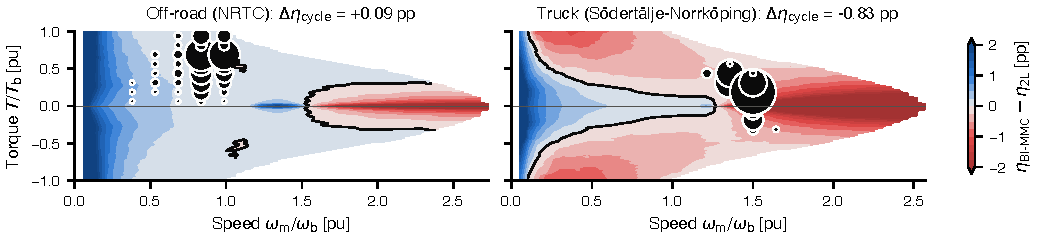
\includegraphics[width=\linewidth]{figures/cycle_maps_soc50.pdf}
\caption{Efficiency difference BI-MMC $-$ 2L (semiconductors and battery) over the torque--speed map at \SI{50}{\percent} SOC, for the off-road machine and the heavy-duty truck. Solid line: $\Delta\eta=0$. Dots: cycle energy $|P|\Delta t$ per bin; dot area is proportional to the share of the cycle energy.}
\label{fig:maps}
\end{figure}

\Cref{fig:summary}(a) breaks the cycle losses down. In all applications the BI-MMC cuts semiconductor losses, by \SIrange{37}{80}{\percent} in road, off-road and marine duty and by \SI{26}{\percent} in the train, where 13 series SMs carry the high phase current; switching losses almost vanish and peak junction temperatures drop by \SIrange{6}{25}{\kelvin}. In return, its battery losses are \SIrange{1.6}{4.4}{} times higher. \Cref{fig:summary}(b) condenses this into a design rule: the BI-MMC only gains when nearly all cycle energy is delivered below base speed at moderate to high torque (ship, off-road machine), and even then the gain is about \SI{0.1}{\pp}. The passenger car and the city bus lose \SIrange{0.5}{0.6}{\pp}: the car has \SI{62}{\percent} of its energy below base speed, but its light WLTC loads keep the 2L losses low. The truck (\SI{-0.83}{\pp}) and the regional train (\SI{-1.7}{\pp}) spend most of the cycle in field weakening. Low SOC deepens field weakening and penalises the BI-MMC; the off-road gain nearly vanishes at \SI{20}{\percent} SOC.

\begin{figure}[h]
\centering
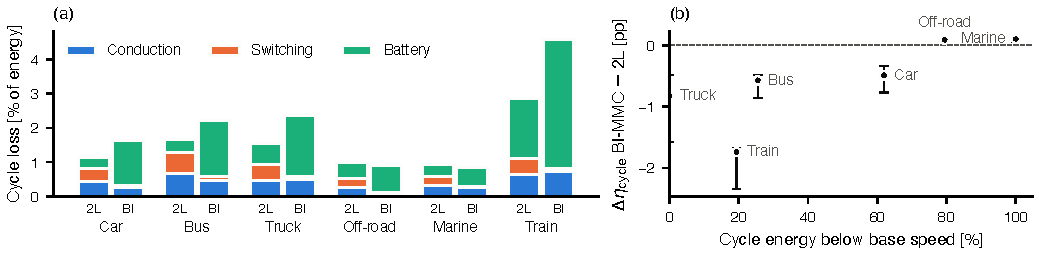
\includegraphics[width=\linewidth]{figures/cycle_summary.pdf}
\caption{(a) Cycle losses by component in percent of the traction energy throughput at \SI{50}{\percent} SOC; (b) cycle efficiency difference BI-MMC $-$ 2L versus the share of cycle energy below base speed (bars: \SIrange{20}{90}{\percent} SOC).}
\label{fig:summary}
\end{figure}

\section{Conclusion and Content of the Final Paper}
The open-source platform puts the efficiency maps and drive-cycle efficiency of an AC battery and a 2L inverter on equal terms. Across six applications, the AC battery cuts semiconductor losses, but the cell losses from the gated phase current offset this: it is at best on par with a SiC 2L inverter at low speed and clearly worse in field weakening (trucks, trains). The platform will be released as open source; the final paper adds a sensitivity study.

\printbibliography
\end{document}
